%----------------------------------------------------------------------
\section{Hyperband}

%-----------------------------------------------------------------------

\begin{frame}{Adaptive Hyperparameter Optimization}
\begin{columns}[T]

\begin{column}{.45\textwidth}
    \begin{itemize}
        \item Idea: Allocate more resources to promising configurations, eliminate poor ones.
        \pause
    \end{itemize}
\end{column}
    \begin{column}{.45\linewidth}
    \begin{figure}
    \centering
    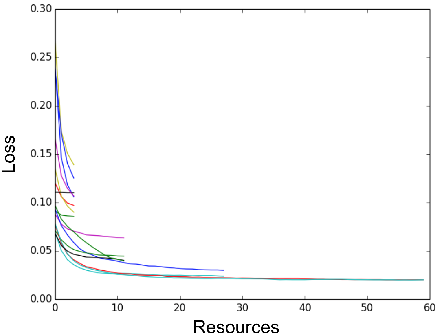
\includegraphics[width=0.9\linewidth]{images/hyperband/Figure_1_2.png}
\end{figure}
    \end{column}
    \end{columns}
    \begin{columns}
    
    \begin{column}{.45\linewidth}
    \vspace{-9em}
    \begin{itemize}
	\item Result: Examine more configurations.
	\pause
	\item Resources:
	\pause
	\begin{itemize}
	    \item Runtime
	    \pause
	    \item Number of epochs
	    \pause
	    \item Number of trees
	    \pause
	    \item Data subset size
	    \pause
	    \item Number of cross validation folds
	    
	    \item ...
	\end{itemize}
\end{itemize}
\end{column}

\begin{column}{.45\textwidth}

\end{column}

\end{columns}

\end{frame}

%-----------------------------------------------------------------------

\begin{frame}{Successive Halving(SH)}
\begin{columns}

\begin{column}{.45\textwidth}
\vspace{-1em}
\begin{itemize}
    \item Simple technique
    \item Does not make strong assumptions on the convergence of the underlying algorithm.
    %\item Bandit-based approach to hyperparameter optimization.
    \pause
    \item Uniformly allocate a budget to a set.
    \pause
\end{itemize}
\end{column}

\begin{column}{.5\textwidth}
\begin{figure}
    \centering
    \vspace{2em}
    \only<3>{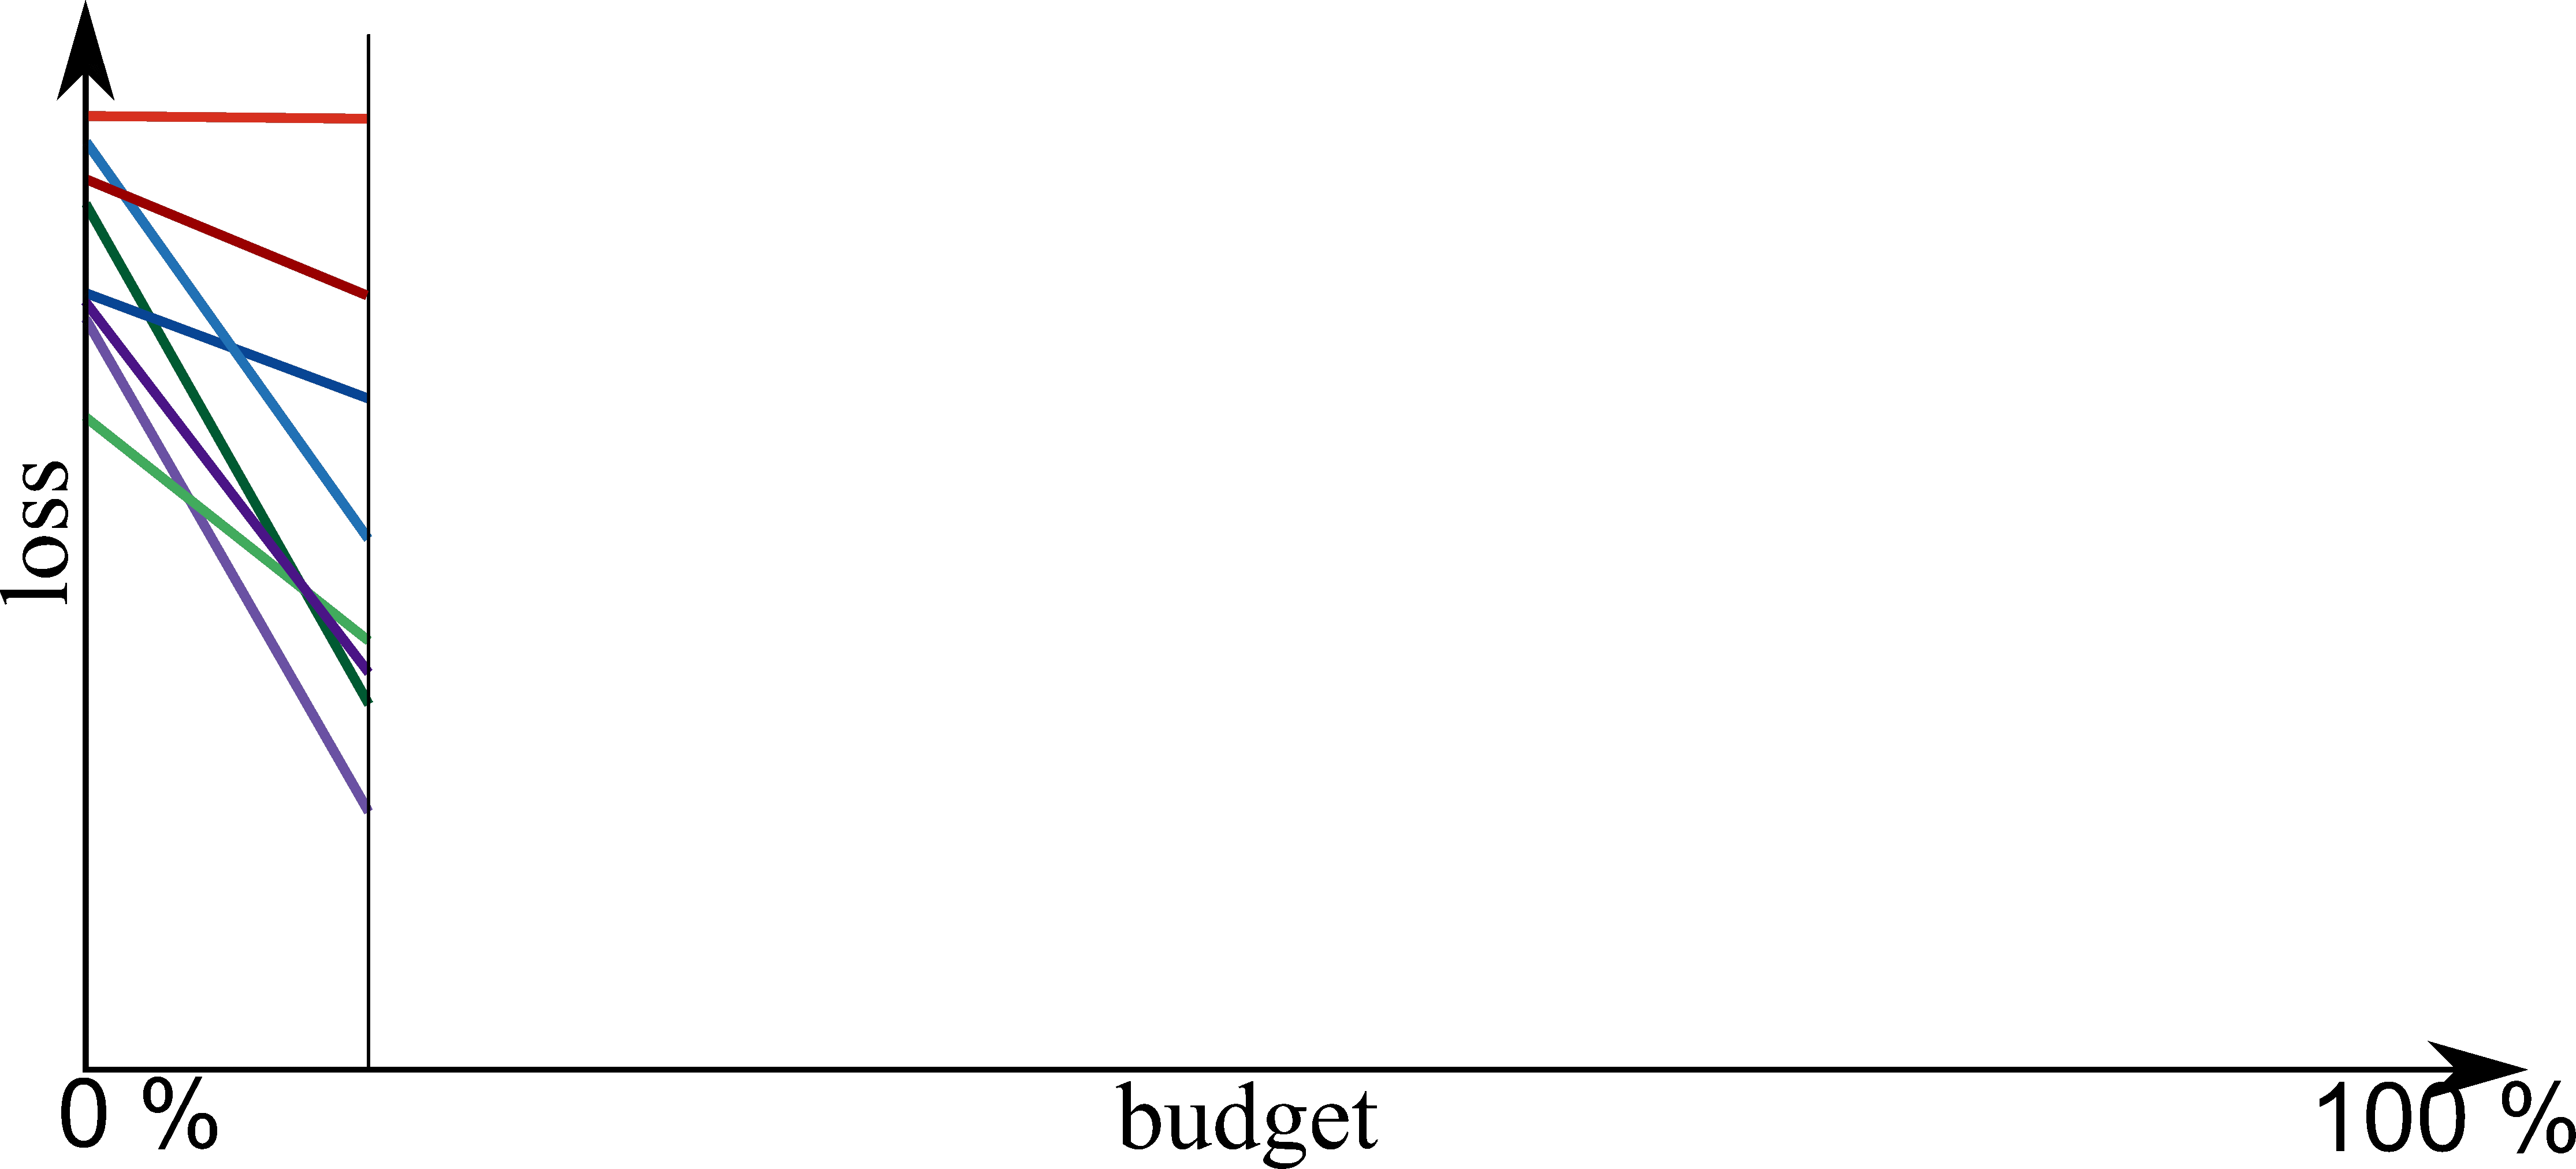
\includegraphics[width=\linewidth]{images/hyperband/SH-1.png}}
    \only<4>{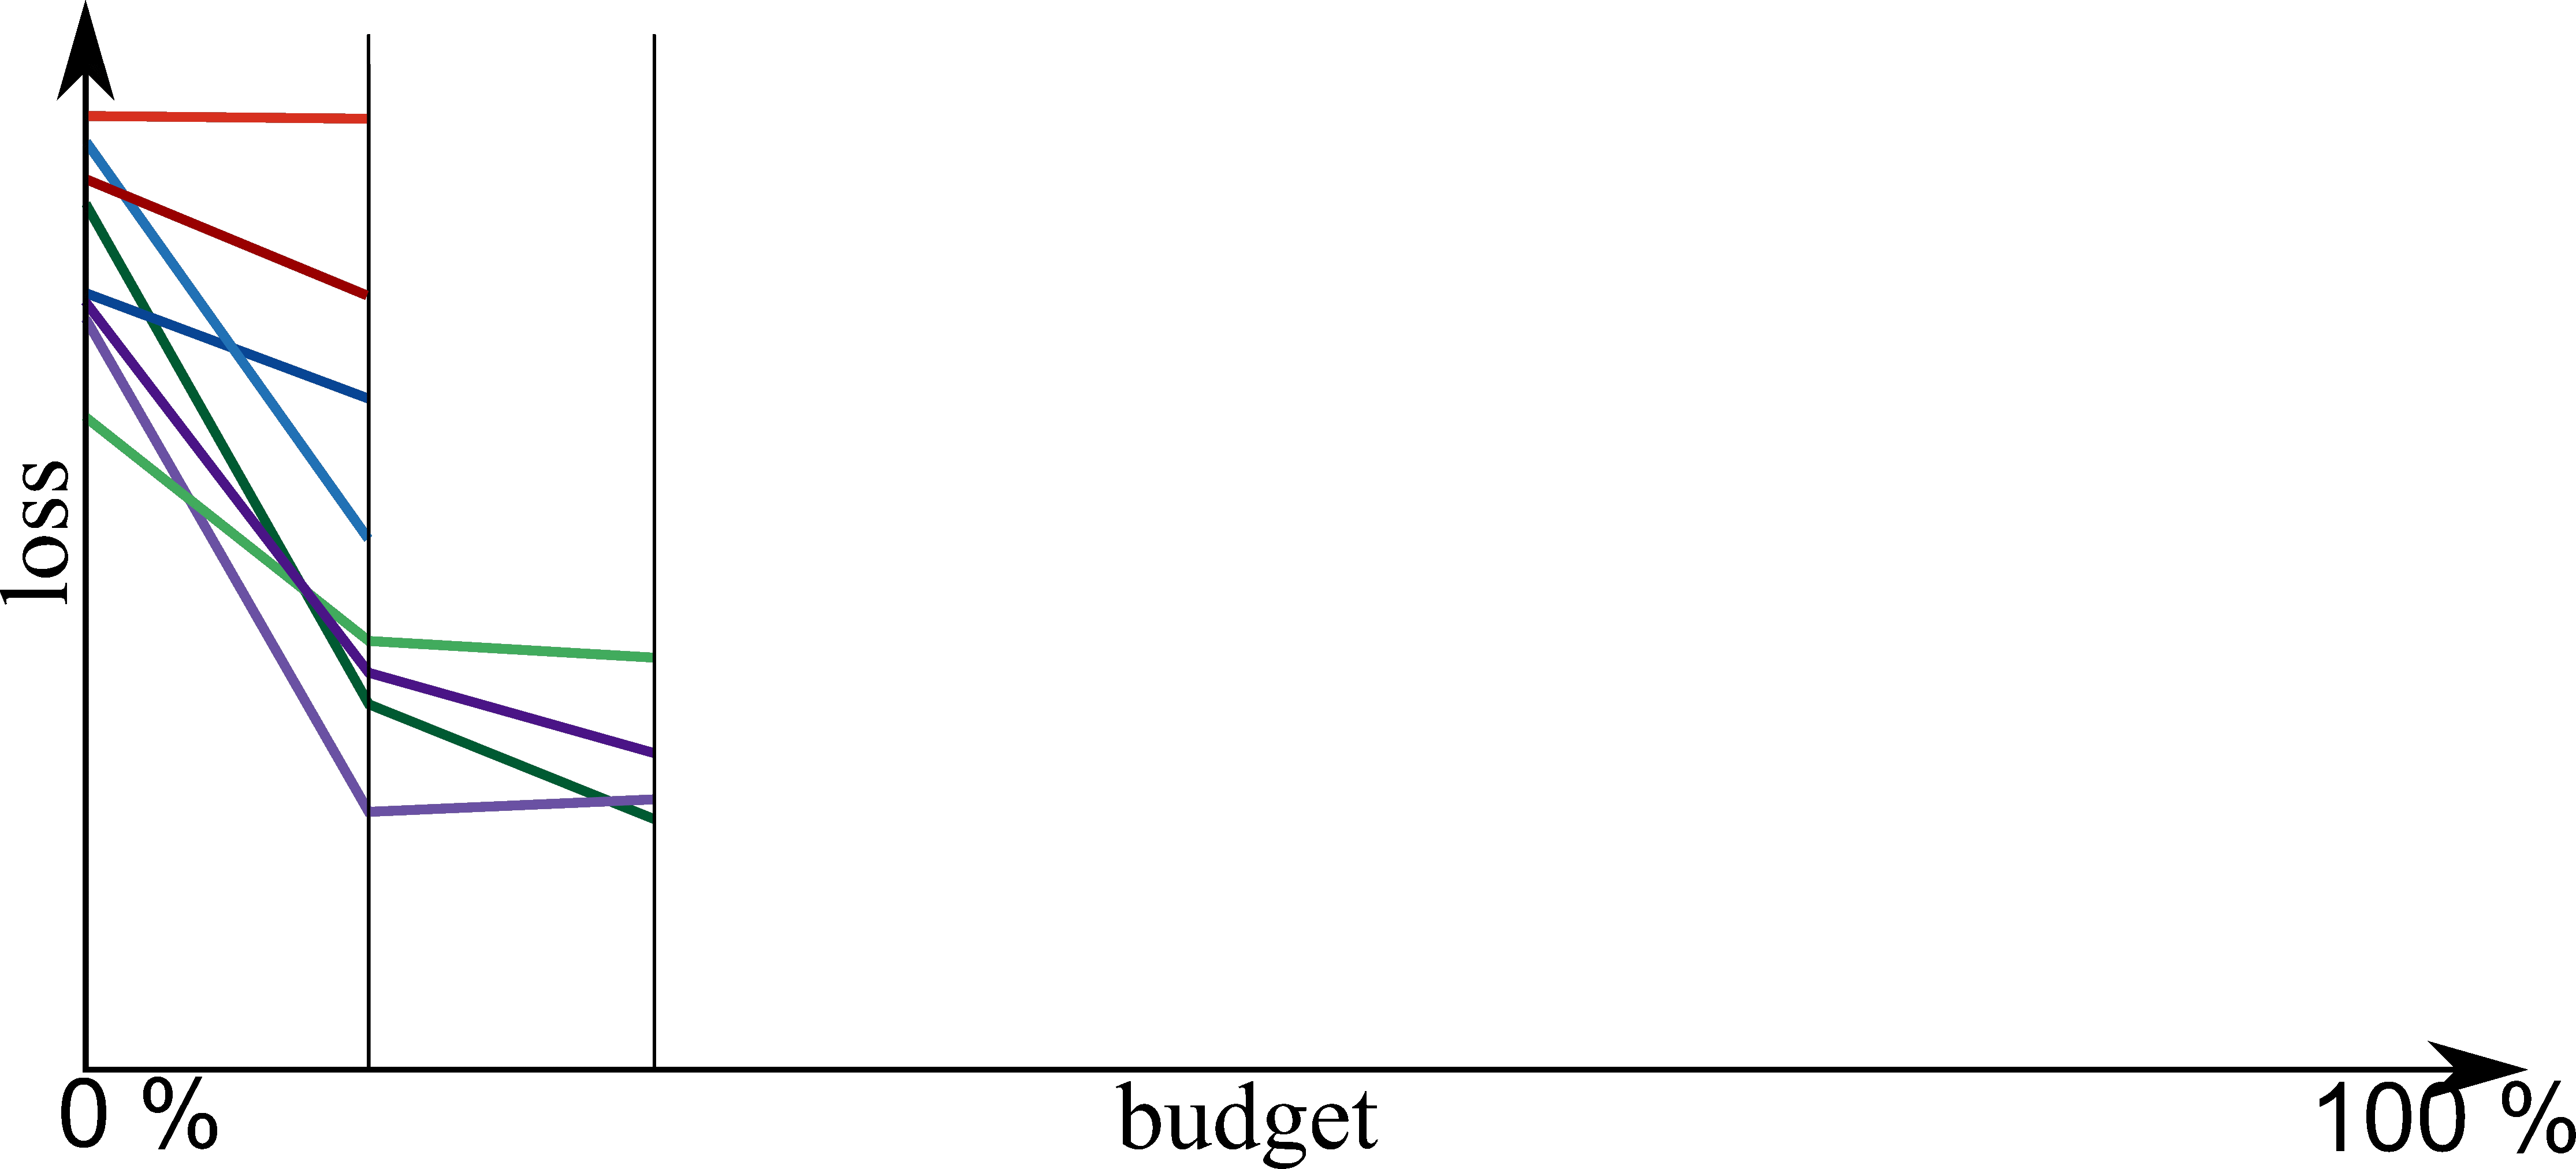
\includegraphics[width=\linewidth]{images/hyperband/SH-2.png}}
    \only<5>{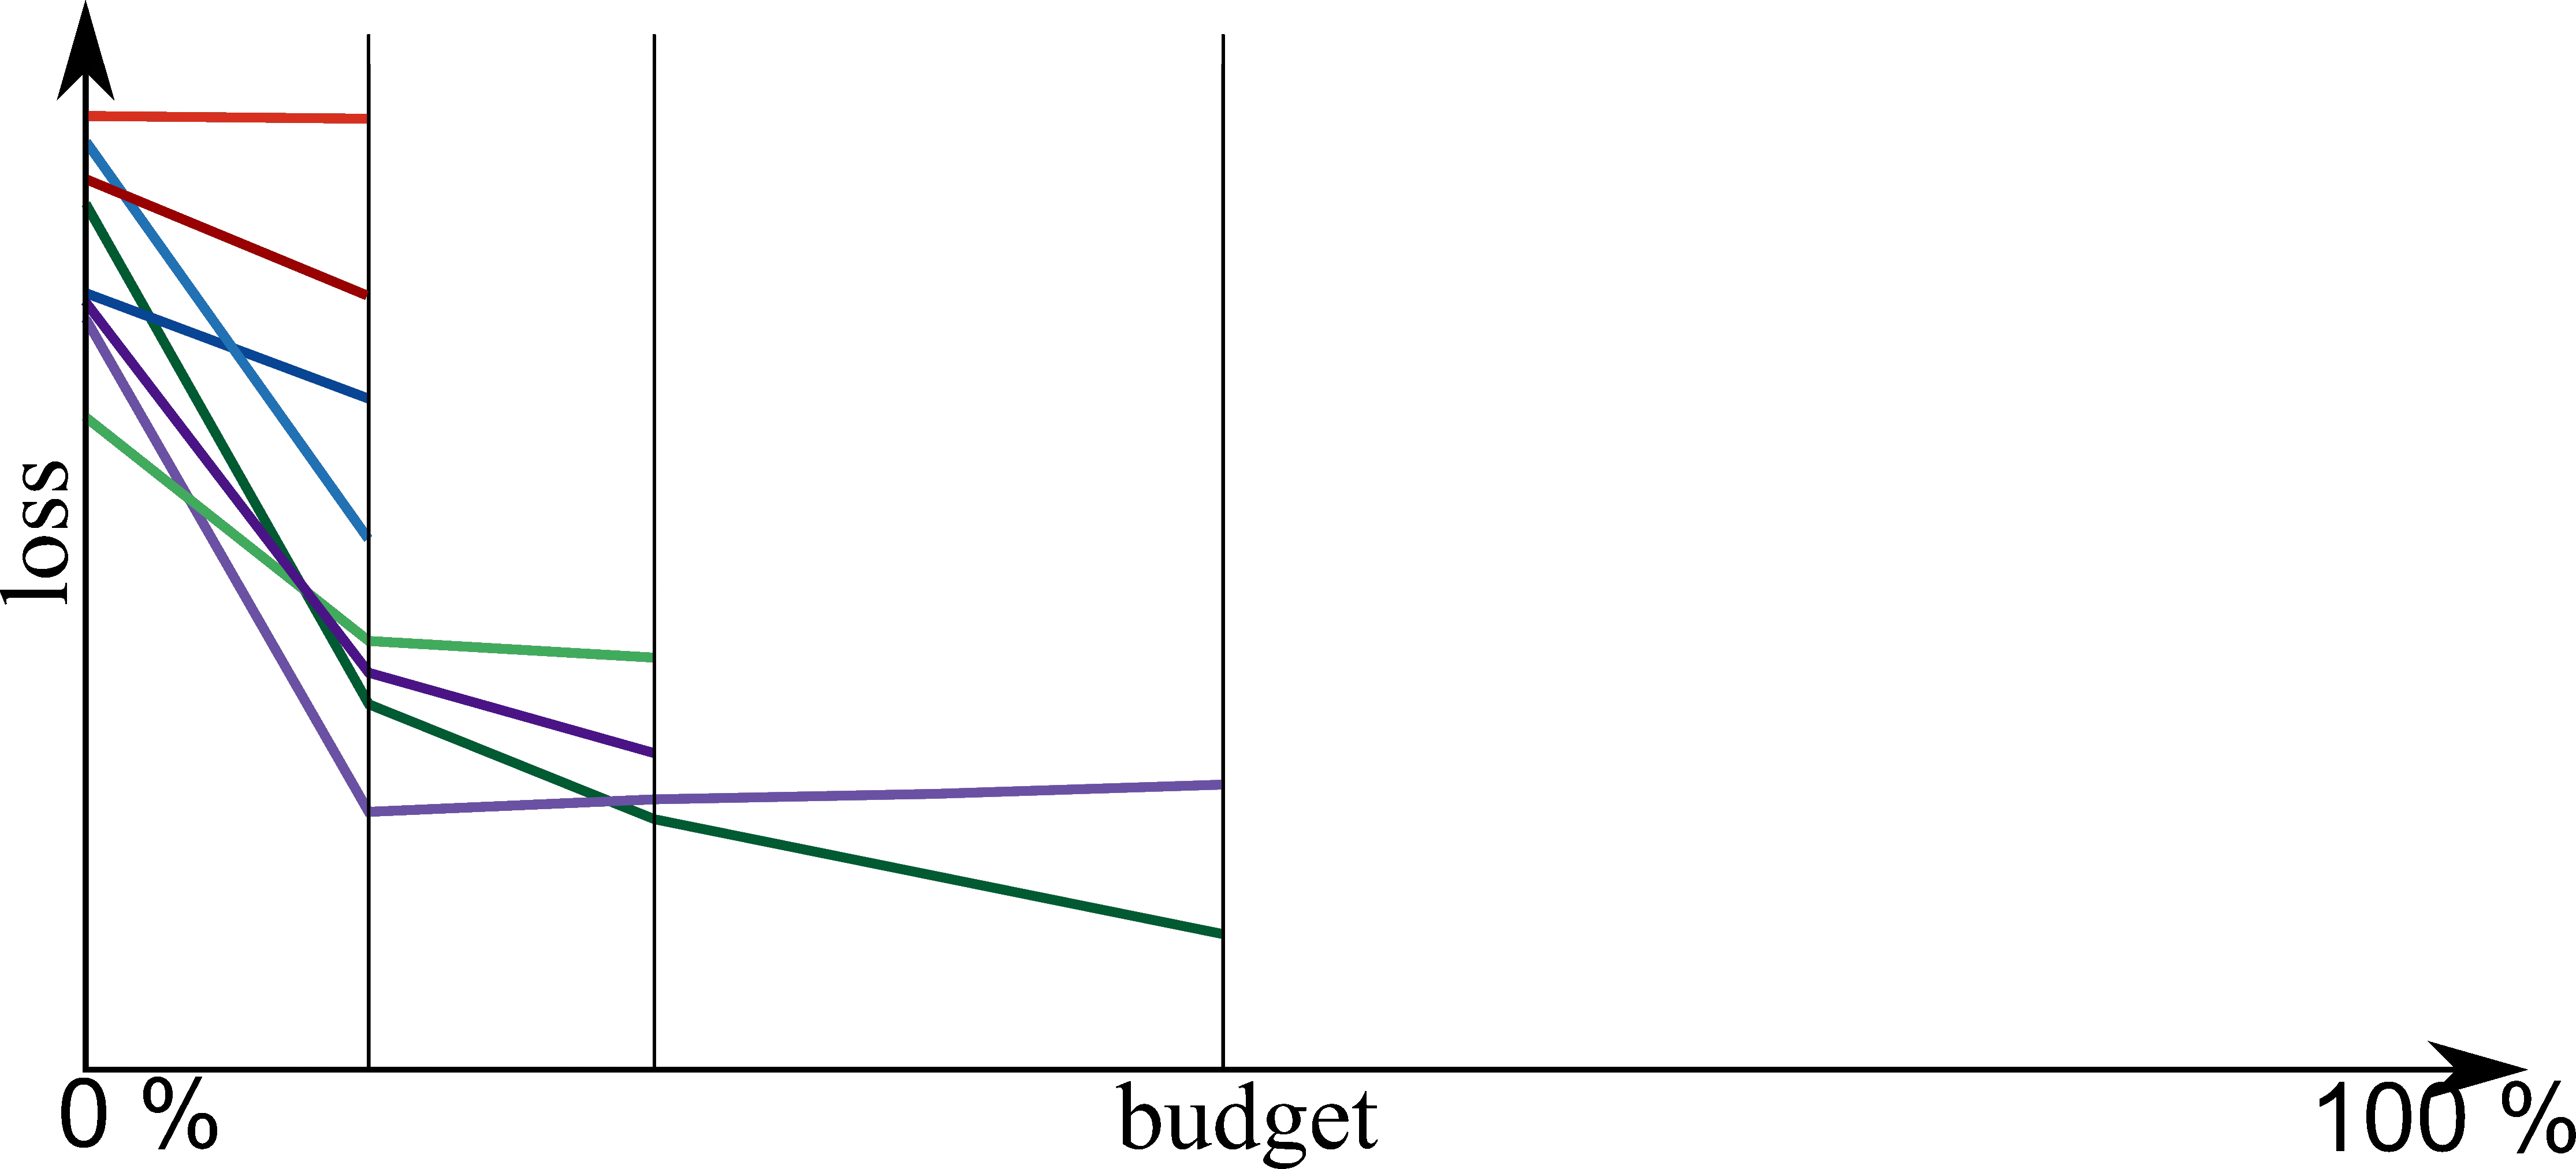
\includegraphics[width=\linewidth]{images/hyperband/SH-3.png}}
    \only<6>{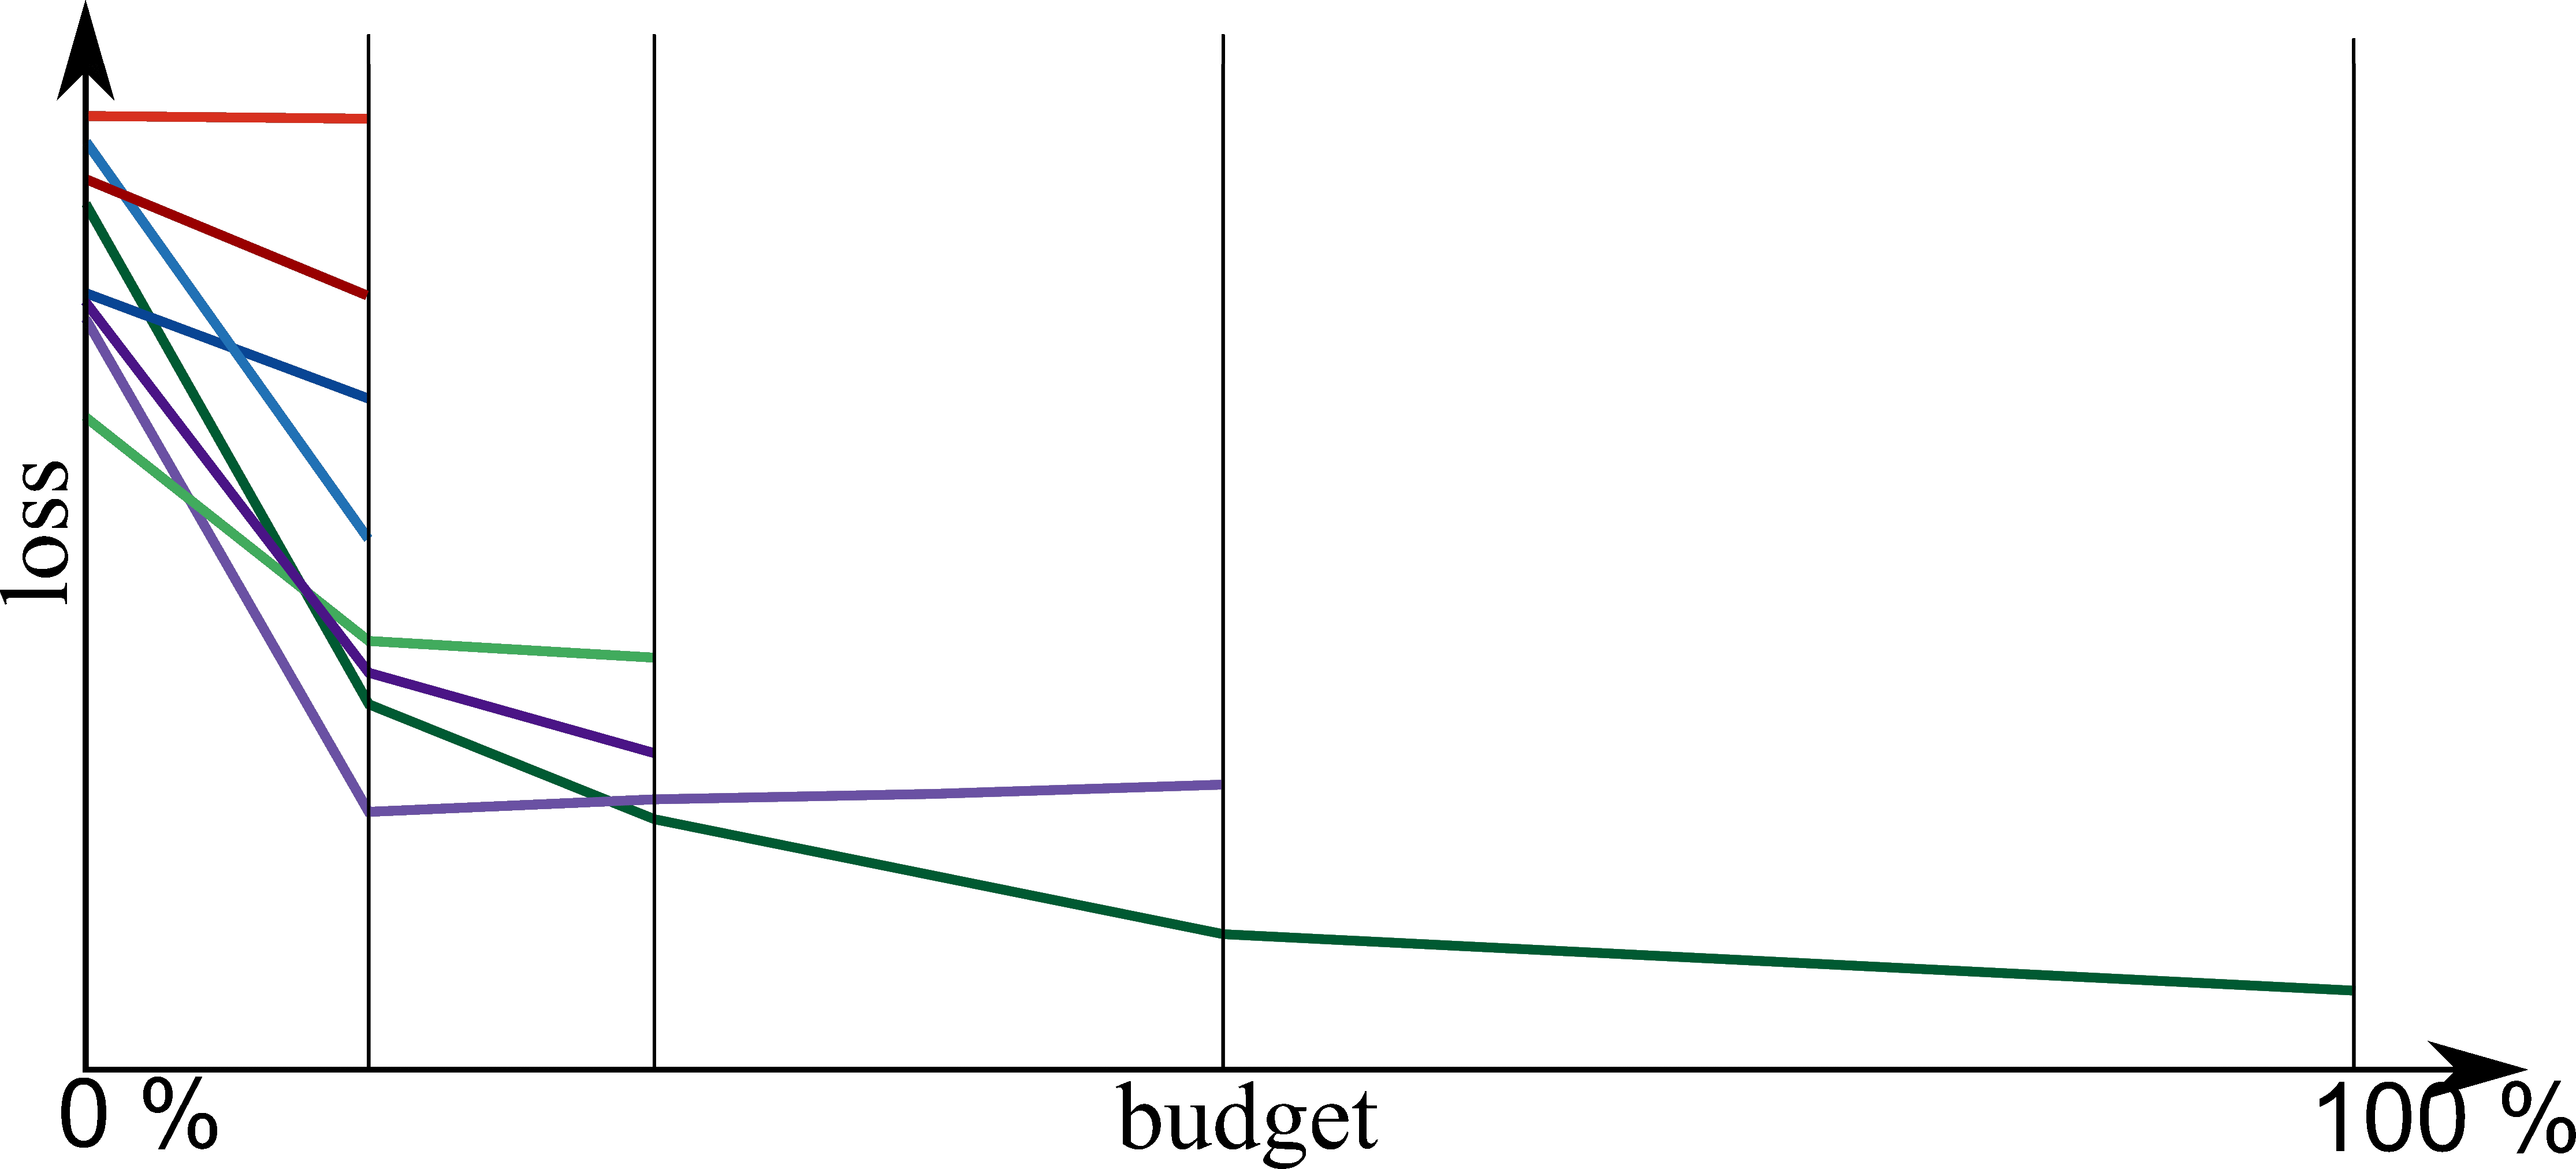
\includegraphics[width=\linewidth]{images/hyperband/SH-4.png}}

\end{figure}
\end{column}
\end{columns}
\vspace{-5em}
\begin{columns}
\begin{column}{.45\textwidth}
Given a budget $B$ and the number of configurations $n$ as an input:
\pause
\begin{itemize}
    \item Evaluate the performance of all configurations.
    \pause
    \item Throw out the worst performing half.
    \pause
    \item Repeat until one configuration remains.

\end{itemize}
\end{column}

\begin{column}{.45\textwidth}
\end{column}

\end{columns}

\end{frame}

%-----------------------------------------------------------------------
%-----------------------------------------------------------------------

\begin{frame}{Successive Halving(SH): Algorithm}
\begin{algorithm}[H]
    %\DontPrintSemicolon
    \LinesNumbered
    \SetAlgoLined
    \setcounter{AlgoLine}{0}
    \SetKwInOut{Input}{Input}
    \DeclarePairedDelimiter\ceil{\lceil}{\rceil}
    \DeclarePairedDelimiter\floor{\lfloor}{\rfloor}
    \DeclarePairedDelimiter\abs{\lvert}{\rvert}
    
    \Input{ initial budget $b_0,$ maximum budget $b_{max},$ set of $n$ configurations $C=\{\conf_1, \conf_2,\dots, \conf_{n}\}$}
    $b=b_0$\\
    \While{$b\leq b_{max}$}{
    $L=\{\Tilde{\cost}(\conf,b):\conf \in C\}$;\
    
    $C=top_{k}(C,L,\lfloor\lvert C \rvert\ / \eta \rfloor)$;\
    
    $b=\eta \cdot b$;\
    }
    
 
        
    
    \caption{Pseudocode for SuccessiveHalving used by Hyperband as a subroutine}
\end{algorithm}

\end{frame}

%-----------------------------------------------------------------------

\begin{frame}{\emph{"n versus B/n" Problem}}
\begin{columns}

\begin{column}{.45\linewidth}
\begin{itemize}
    \item SH requires $B$ and $n$ as an input.
    \pause
    \item Given finite $B$, $B/n$ resources are allocated across the configurations.
    \pause
\end{itemize}
\end{column}

\begin{column}{.45\linewidth}

\begin{figure}
    \centering
    \vspace{2em}
    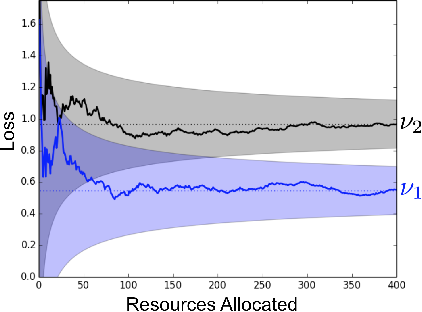
\includegraphics[width=0.9\linewidth]{images/intro/differetiatingConfigurations.png}
    \pause
\end{figure}
\end{column}
\end{columns}
\vspace{-10em}
\begin{columns}

\begin{column}{.45\linewidth}
\begin{itemize}
    \item Configurations need enough minimal resources to differentiate between them in terms of quality.
    \pause
    \item Issue: Optimal allocation strategy is unknown in practice.
    \pause
    \item Idea: Perform grid search over a feasible set of tuples of $n$ and minimal resource $r$. (Hyperband) 
\end{itemize}
\end{column}

\begin{column}{.45\linewidth}

\end{column}
    
\end{columns}
    
\end{frame}

%-----------------------------------------------------------------------
\begin{frame}{Hyperband}
\begin{itemize}
    \item Issue of successive halving (for a fixed B):
    \begin{itemize}
        \item Do you want to run many configurations with aggressive rejection?
        \item Or: Do you want to run few configurations with non-aggressive rejection?
    \end{itemize}
    \item Ideas:
    \begin{itemize}
        \item Add an outer loop to try different trade-offs between $\#$configurations and budget.
        \item Add further parameter: proportion of configurations discarded in each round of successive halving
    \end{itemize}
    \item Starts with many configurations that gets aggressively rejected.
    \item In later iterations, few configurations with more budget each.
    \item Returns: configuration with the smallest intermediate loss seen so far.
\end{itemize}
\end{frame}

%-----------------------------------------------------------------------

\begin{frame}{Hyperband: Algorithm}
\begin{minipage}{0.75\textwidth}
\begin{algorithm}[H]
    %\DontPrintSemicolon
    \LinesNumbered
    \SetAlgoLined
    \setcounter{AlgoLine}{0}
    \DeclarePairedDelimiter\ceil{\lceil}{\rceil}
    \DeclarePairedDelimiter\floor{\lfloor}{\rfloor}
    
    \Input{budgets $b_{min}$ and $b_{max}, \eta$}
    
    $s_{max}=\floor*{\log_{\eta}\frac{b_{max}}{b_{min}}}$;\
    
    \For{$s\in \{s_{max}, s_{max}-1, \dots, 0\}$}
    {
        sample $\eta=\lceil\frac{s_{max}+1}{s+1} \cdot\eta^{s}\rceil$;\
        
        run SH on them with $\eta^{s}\cdot b_{max}$;\
    }
 
        
    
    \caption{Pseudocode for Hyperband using SuccessiveHalving (SH) as a subroutine}
\end{algorithm}
\end{minipage}
\end{frame}
%-----------------------------------------------------------------------
\begin{frame}{Hyperband}
\begin{figure}
    \centering
    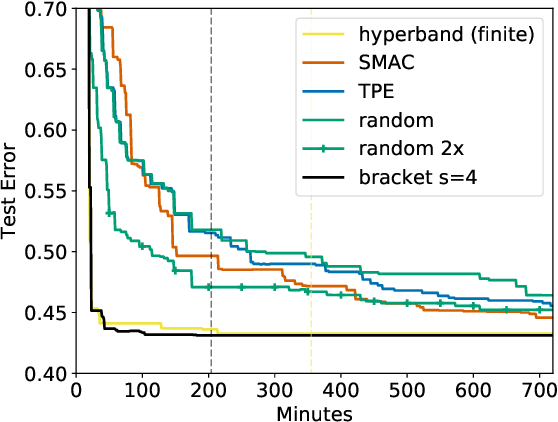
\includegraphics[width=0.6\textwidth]{images/hyperband/Figure_experiments.png}
\end{figure}

    
\end{frame}

%-----------------------------------------------------------------------
%-----------------------------------------------------------------------
\begin{frame}{Random Search vs. Hyperband}
\begin{figure}
    \centering
    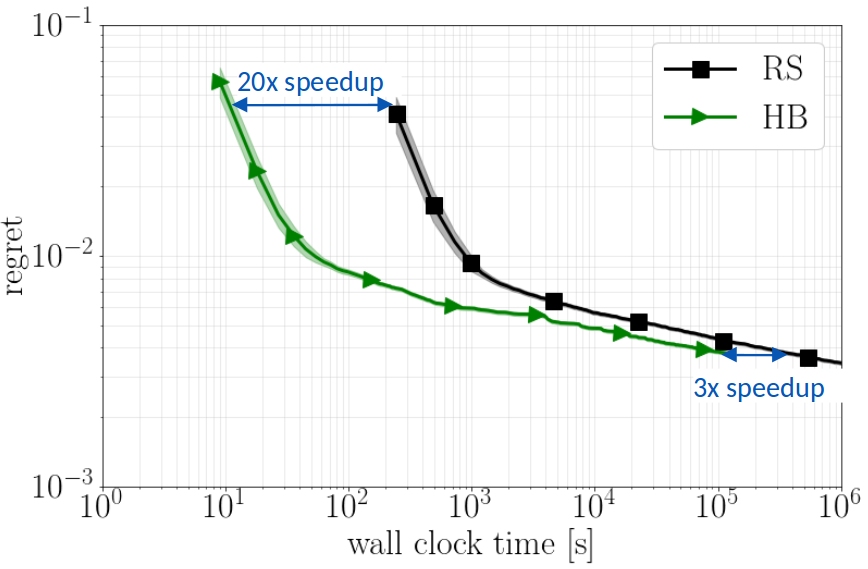
\includegraphics[width=0.7\textwidth]{images/hyperband/bohb_2.png}
\end{figure}

    
\end{frame}

%-----------------------------------------------------------------------